\subsection{Overshooting Convection Variants}
\frame{\tableofcontents[currentsubsection]}

\frame{\frametitle{We'd like to try to include non-linear diffusion for handling composition-dependent opacities.}
	\begin{overprint}
		\only<1>{
			\begin{equation}
				\kappa_{T}\left(z, \mu\right) = \kappa_{0}\left(z\right)+\kappa_{1}\mu
			\end{equation}	
			We assume that the largest variations will be in the z-direction, so we propose calculating
			\begin{equation}
				\kappa_{1,z}\left(z\right) = \kappa_{1}\overline{\mu}\left(z\right),
			\end{equation}	
			and adding this to $\kappa_{0}\left(z\right)$ every so many steps.
		}
		\only<2>{
			This works quite well in one-dimensional tests as long as $\kappa_{1}\mu< 0.1\kappa_{0}$.

			However, it fails in two dimensions due to larger variations in the horizontal direction than expected.
		}
	\end{overprint}
}

\frame{\frametitle{Under the Boussinesq approximation, there are three possibilities for an overshooting region.}
	\begin{itemize}
		\item A spatially-dependent thermal expansion coefficient
		\item A spatially-dependent heating term
		\item A spatially-dependent diffusion coefficient
	\end{itemize}
}

\frame{\frametitle{Governing equations \citep{Spiegel1960}}
\begin{overprint}
\only<1>{
Assuming the Boussinesq approximation and an adiabatic temperature gradient (such as appears during a formal derivation of the Boussinesq approximation for a gas) yields
\begin{align}
	\rho_{0}\frac{D}{D{t}}{\mathbf{u}} =& -\nabla p - \left(\rho - \rho_{0}\right) g + \rho_{0}\nu\nabla^{2}\mathbf{u} \\
	\nabla\cdot\mathbf{u} =& 0 \\
	\rho_{0}\frac{D}{D{t}}{T} - \rho_{0}\left.\frac{d}{dz}T\right|_{\mathrm{ad}} =& \rho_{0}\nabla\cdot\kappa_T(z) \nabla T + H\left(z\right) \\
\end{align}}
\only<2>{
Subtracting a static background temperature and non-dimensionalizing yields
\begin{align}
	\frac{D}{D{t}}{\mathbf{u}} =& -\nabla p + \frac{\mathrm{Ra}_{T}}{\mathrm{Pr}}{T} + \nabla^{2}\mathbf{u} \\
	\nabla\cdot\mathbf{u} =& 0 \\
	\frac{D}{D{t}}{T} + w f\left(z\right) =& \nabla\cdot \left(\mathrm{Pr}^{-1}+\kappa_{T}(z)/\kappa_{T,0}\right)\nabla T, \\
\end{align}
where $\kappa_{T}(z)$ is zero in the uniform diffusion case.}
\end{overprint}
}

\frame{\frametitle{We are currently investigating the differences between heating and variable diffusion.}
\begin{overprint}
	\only<1>{
	\begin{figure}[h]
		\centering
		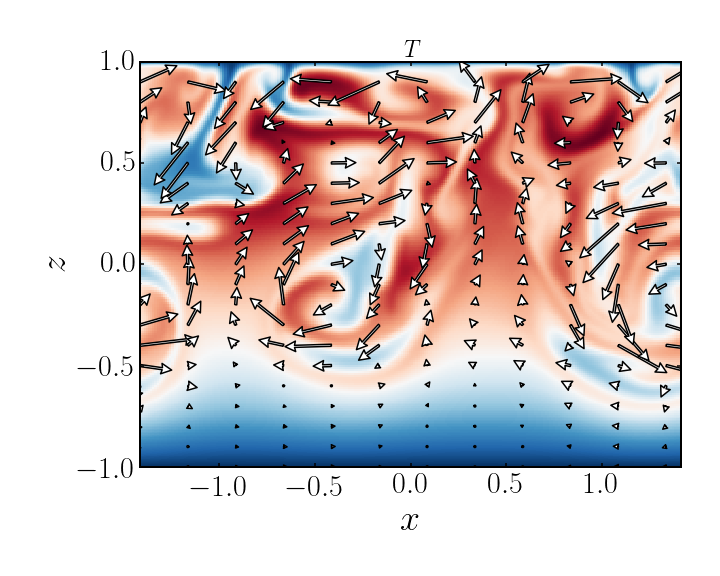
\includegraphics[width=.5\textwidth]{figs/osht_heat.png}
		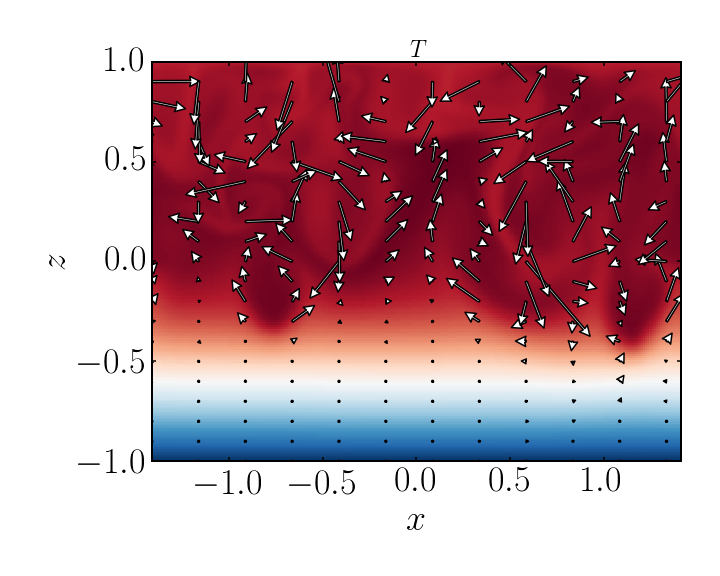
\includegraphics[width=.5\textwidth]{figs/osht_diff.png}
		\label{fig:osht_heat}
	\end{figure}
	}	
	\only<2>{
	\begin{figure}[h]
		\centering
			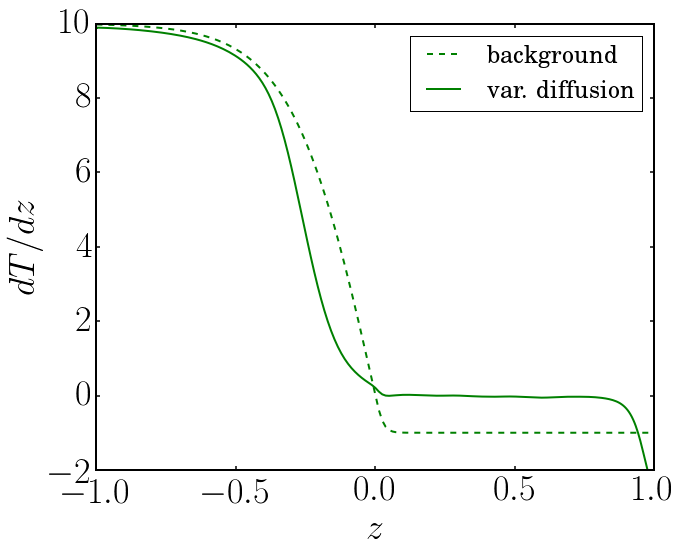
\includegraphics[width=.7\textwidth]{figs/var_diff.png}
		\label{fig:var_vs_heat}
	\end{figure}
	}	
\end{overprint}
}